% =============================================================================
% Appendix D: Player Database Schema
% סכמת בסיס הנתונים של סוכן השחקן
% Standalone chapter with subfiles support
% =============================================================================
\documentclass[../master/main.tex]{subfiles}

\begin{document}

\chapter*{נספח ד': סכמת בסיס הנתונים של סוכן השחקן}
\addcontentsline{toc}{chapter}{נספח ד': סכמת בסיס הנתונים של סוכן השחקן}
\renewcommand{\thehebrewsection}{ד.\arabic{hebrewsection}}
\setcounter{hebrewsection}{0}

\hebrewsection{מבוא}

נספח זה מתאר את סכמת בסיס הנתונים של סוכן השחקן (\en{GmailAsPlayer}). בסיס הנתונים מבוסס על \en{PostgreSQL} ומאורגן בארבע קבוצות לוגיות:

\begin{enumerate}
    \item \textbf{טבלאות שחקן ומצב} --- שמירת מצב השחקן והיסטוריית מעברים
    \item \textbf{טבלאות משחק} --- סשנים, שאלות, תשובות וניחושים
    \item \textbf{טבלאות הודעות וקבצים} --- תיעוד הודעות פרוטוקול ומעקב קבצים
    \item \textbf{טבלאות שידור} --- מעקב אחר הודעות שידור והשהיה/המשך
\end{enumerate}

\textbf{סה``כ טבלאות:} \num{11} (כולל \en{schema\_version})

% =============================================================================
\hebrewsection{דיאגרמת הסכמה}
\label{sec:schema-diagram}
% =============================================================================

איור~\ref{fig:player-db-schema} מציג את מבנה בסיס הנתונים המלא, כולל קשרי מפתחות זרים בין הטבלאות.

\begin{landscape}
\begin{figure}[H]
\centering
\begin{english}
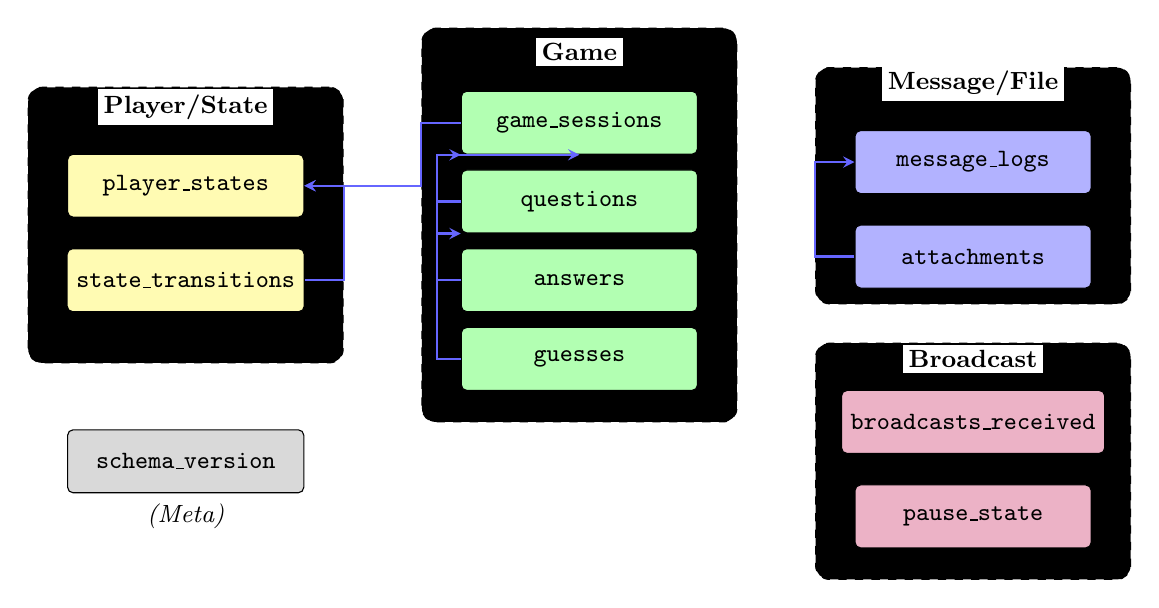
\begin{tikzpicture}[
    table/.style={
        draw, rectangle, rounded corners=2pt,
        minimum width=3cm, minimum height=0.8cm,
        font=\small\ttfamily, align=center
    },
    group/.style={
        draw, dashed, rounded corners=5pt,
        inner sep=8pt, #1
    },
    grouplabel/.style={font=\small\bfseries, fill=white, inner sep=2pt},
    fkarrow/.style={->, >=stealth, thick, blue!60}
]
    % Group 1: Player/State (Yellow)
    \node[group=fill=yellow!15] (g1) at (0,0) [minimum width=4cm, minimum height=3.5cm] {};
    \node[grouplabel] at (0,1.5) {Player/State};
    \node[table, fill=yellow!30] (ps) at (0,0.5) {player\_states};
    \node[table, fill=yellow!30] (st) at (0,-0.7) {state\_transitions};

    % Group 2: Game (Green)
    \node[group=fill=green!15] (g2) at (5,0) [minimum width=4cm, minimum height=5cm] {};
    \node[grouplabel] at (5,2.2) {Game};
    \node[table, fill=green!30] (gs) at (5,1.3) {game\_sessions};
    \node[table, fill=green!30] (q) at (5,0.3) {questions};
    \node[table, fill=green!30] (a) at (5,-0.7) {answers};
    \node[table, fill=green!30] (gu) at (5,-1.7) {guesses};

    % Group 3: Message/File (Blue)
    \node[group=fill=blue!15] (g3) at (10,0.5) [minimum width=4cm, minimum height=3cm] {};
    \node[grouplabel] at (10,1.8) {Message/File};
    \node[table, fill=blue!30] (ml) at (10,0.8) {message\_logs};
    \node[table, fill=blue!30] (at) at (10,-0.4) {attachments};

    % Group 4: Broadcast (Purple)
    \node[group=fill=purple!15] (g4) at (10,-3) [minimum width=4cm, minimum height=3cm] {};
    \node[grouplabel] at (10,-1.7) {Broadcast};
    \node[table, fill=purple!30] (br) at (10,-2.5) {broadcasts\_received};
    \node[table, fill=purple!30] (pau) at (10,-3.7) {pause\_state};

    % Meta table
    \node[table, fill=gray!30] (sv) at (0,-3) {schema\_version};
    \node[font=\small\itshape] at (0,-3.7) {(Meta)};

    % Foreign Key relationships
    \draw[fkarrow] (st.east) -- ++(0.5,0) |- (ps.east);
    \draw[fkarrow] (gs.west) -- ++(-0.5,0) |- (ps.east);
    \draw[fkarrow] (q.west) -- ++(-0.3,0) |- (gs.south west);
    \draw[fkarrow] (a.west) -- ++(-0.3,0) |- (q.south west);
    \draw[fkarrow] (gu.west) -- ++(-0.3,0) |- (gs.south);
    \draw[fkarrow] (at.west) -- ++(-0.5,0) |- (ml.west);

\end{tikzpicture}
\end{english}
\caption{סכמת בסיס הנתונים של סוכן השחקן --- \num{11} טבלאות בארבע קבוצות לוגיות}
\label{fig:player-db-schema}
\end{figure}
\end{landscape}

\hebrewsubsection{מקרא הדיאגרמה}

\begin{itemize}
    \item \textbf{צהוב (\en{PK})} --- מפתח ראשי (\en{Primary Key})
    \item \textbf{כחול בהיר (\en{FK})} --- מפתח זר (\en{Foreign Key})
    \item \textbf{חצים} --- קשרי מפתחות זרים בין טבלאות
    \item \textbf{\en{UNIQUE}} --- אילוץ ייחודיות
\end{itemize}

% =============================================================================
\needspace{10\baselineskip}
\hebrewsection{טבלאות שחקן ומצב}
\label{sec:player-tables}
% =============================================================================

\hebrewsubsection{טבלת \en{player\_states}}

טבלה זו היא הטבלה המרכזית לניהול מצב השחקן. כל שורה מייצגת שחקן רשום במערכת.

\begin{fancytable}{lHH}{עמודות טבלת \en{player\_states}}
\label{tab:player-states}
עמודה & סוג & תיאור \\
\en{id} & \en{SERIAL PK} & מזהה אוטומטי \\
\en{player\_email} & \en{VARCHAR UNIQUE} & כתובת אימייל השחקן \\
\en{player\_name} & \en{VARCHAR} & שם תצוגה \\
\en{current\_state} & \en{VARCHAR} & מצב נוכחי במכונת המצבים \\
\en{current\_game\_id} & \en{VARCHAR} & מזהה משחק פעיל \\
\en{current\_book} & \en{VARCHAR} & שם הספר הנוכחי \\
\en{registration\_id} & \en{VARCHAR} & מזהה טרנזקציית רישום \\
\en{last\_activity} & \en{TIMESTAMP} & זמן פעילות אחרון \\
\en{created\_at} & \en{TIMESTAMP} & זמן יצירת הרשומה \\
\end{fancytable}

\textbf{מצבי השחקן האפשריים:}
\begin{itemize}
    \item \en{IDLE} --- לא במשחק
    \item \en{REGISTERING} --- רישום בתהליך
    \item \en{REGISTERED} --- רשום בליגה
    \item \en{WAITING\_MATCH} --- ממתין לשיבוץ משחק
    \item \en{IN\_GAME} --- פעיל במשחק
    \item \en{ANSWERING\_QUESTIONS} --- עונה על שאלות
    \item \en{MAKING\_GUESS} --- מבצע ניחוש סופי
\end{itemize}

\hebrewsubsection{טבלת \en{state\_transitions}}

טבלת היסטוריה למעקב אחר מעברי מצבים. משמשת לניפוי שגיאות ואנליטיקה.

\begin{fancytable}{lHH}{עמודות טבלת \en{state\_transitions}}
\label{tab:state-transitions}
עמודה & סוג & תיאור \\
\en{id} & \en{SERIAL PK} & מזהה אוטומטי \\
\en{player\_email} & \en{VARCHAR} & כתובת אימייל השחקן \\
\en{from\_state} & \en{VARCHAR} & מצב קודם \\
\en{to\_state} & \en{VARCHAR} & מצב חדש \\
\en{event} & \en{VARCHAR} & האירוע שגרם למעבר \\
\en{transition\_metadata} & \en{JSONB} & מטא-דאטה נוסף \\
\end{fancytable}

% =============================================================================
\needspace{10\baselineskip}
\hebrewsection{טבלאות משחק}
\label{sec:game-tables}
% =============================================================================

\hebrewsubsection{טבלת \en{game\_sessions}}

כל שורה מייצגת סשן משחק אחד. זוהי טבלת האב לשאלות, תשובות וניחושים.

\begin{fancytable}{lHH}{עמודות טבלת \en{game\_sessions}}
\label{tab:game-sessions}
עמודה & סוג & תיאור \\
\en{id} & \en{SERIAL PK} & מזהה אוטומטי \\
\en{game\_id} & \en{VARCHAR UNIQUE} & מזהה סשן המשחק \\
\en{player\_email} & \en{VARCHAR FK} & מפתח זר ל-\en{player\_states} \\
\en{book\_name} & \en{VARCHAR} & שם הספר לניחוש \\
\en{domain} & \en{VARCHAR} & תחום אסוציאטיבי \\
\en{is\_completed} & \en{BOOLEAN} & האם המשחק הסתיים \\
\en{result\_correct} & \en{BOOLEAN} & האם הניחוש נכון \\
\en{result\_score} & \en{DECIMAL} & ציון סופי \\
\en{started\_at} & \en{TIMESTAMP} & זמן תחילת המשחק \\
\end{fancytable}

\hebrewsubsection{טבלת \en{questions}}

שומרת את \num{21} השאלות שהתקבלו מהשופט בכל משחק.

\begin{fancytable}{lHH}{עמודות טבלת \en{questions}}
\label{tab:questions}
עמודה & סוג & תיאור \\
\en{id} & \en{SERIAL PK} & מזהה אוטומטי \\
\en{game\_id} & \en{VARCHAR FK} & מפתח זר ל-\en{game\_sessions} \\
\en{question\_number} & \en{INTEGER} & מספר השאלה (\en{1--21}) \\
\en{question\_text} & \en{TEXT} & טקסט השאלה \\
\en{options} & \en{JSONB} & אפשרויות בחירה \\
\end{fancytable}

\hebrewsubsection{טבלת \en{answers}}

שומרת את תשובות השחקן לכל אחת מ-\num{21} השאלות.

\begin{fancytable}{lHH}{עמודות טבלת \en{answers}}
\label{tab:answers}
עמודה & סוג & תיאור \\
\en{id} & \en{SERIAL PK} & מזהה אוטומטי \\
\en{game\_id} & \en{VARCHAR FK} & מפתח זר ל-\en{game\_sessions} \\
\en{question\_number} & \en{INTEGER} & מספר השאלה \\
\en{selected\_option} & \en{VARCHAR} & התשובה שנבחרה \\
\end{fancytable}

\hebrewsubsection{טבלת \en{guesses}}

שומרת את הניחוש הסופי של השחקן (סוכן ה-\en{AI}) --- משפט פתיחה ומילה אסוציאטיבית.

\begin{fancytable}{lHH}{עמודות טבלת \en{guesses}}
\label{tab:guesses}
עמודה & סוג & תיאור \\
\en{id} & \en{SERIAL PK} & מזהה אוטומטי \\
\en{game\_id} & \en{VARCHAR FK UNIQUE} & מפתח זר ל-\en{game\_sessions} \\
\en{opening\_sentence} & \en{TEXT} & משפט הפתיחה המנוחש \\
\en{sentence\_justification} & \en{TEXT} & נימוק לניחוש המשפט \\
\en{associative\_word} & \en{VARCHAR} & המילה האסוציאטיבית \\
\en{confidence} & \en{DECIMAL} & רמת ביטחון \\
\en{strategy\_used} & \en{VARCHAR} & אסטרטגיית ה-\en{AI} \\
\end{fancytable}

% =============================================================================
\needspace{10\baselineskip}
\hebrewsection{טבלאות הודעות וקבצים}
\label{sec:message-tables}
% =============================================================================

\hebrewsubsection{טבלת \en{message\_logs}}

תיעוד כל הודעות הפרוטוקול --- נכנסות ויוצאות.

\begin{fancytable}{lHH}{עמודות טבלת \en{message\_logs}}
\label{tab:message-logs}
עמודה & סוג & תיאור \\
\en{id} & \en{SERIAL PK} & מזהה אוטומטי \\
\en{gmail\_id} & \en{VARCHAR UNIQUE} & מזהה הודעת \en{Gmail} \\
\en{thread\_id} & \en{VARCHAR} & מזהה שרשור \\
\en{direction} & \en{VARCHAR} & כיוון: \en{IN} או \en{OUT} \\
\en{message\_type} & \en{VARCHAR} & סוג הודעת הפרוטוקול \\
\en{transaction\_id} & \en{VARCHAR} & מזהה טרנזקציה \\
\en{payload} & \en{JSONB} & תוכן ההודעה המלא \\
\en{game\_id} & \en{VARCHAR} & מזהה משחק משויך \\
\en{processed} & \en{BOOLEAN} & סטטוס עיבוד \\
\end{fancytable}

\hebrewsubsection{טבלת \en{attachments}}

מעקב אחר קבצי \en{JSON} מצורפים להודעות הפרוטוקול.

\begin{fancytable}{lHH}{עמודות טבלת \en{attachments}}
\label{tab:attachments}
עמודה & סוג & תיאור \\
\en{id} & \en{SERIAL PK} & מזהה אוטומטי \\
\en{internal\_filename} & \en{VARCHAR UNIQUE} & שם קובץ פנימי \\
\en{original\_filename} & \en{VARCHAR} & שם קובץ מקורי \\
\en{message\_id} & \en{VARCHAR} & מזהה הודעת \en{Gmail} \\
\en{mime\_type} & \en{VARCHAR} & סוג \en{MIME} \\
\en{size\_bytes} & \en{INTEGER} & גודל בבתים \\
\end{fancytable}

% =============================================================================
\hebrewsection{טבלת מעקב הודעות}
\label{sec:user-messages-table}
% =============================================================================

\hebrewsubsection{טבלת \en{user\_messages}}

טבלה קריטית למעקב אחר בקשות ותגובות. מאפשרת זיהוי תגובות חסרות ומניעת שליחה כפולה.

\begin{fancytable}{lHH}{עמודות טבלת \en{user\_messages}}
\label{tab:user-messages}
עמודה & סוג & תיאור \\
\en{id} & \en{SERIAL PK} & מזהה אוטומטי \\
\en{message\_id} & \en{UUID UNIQUE} & מזהה הודעה ייחודי \\
\en{correlation\_id} & \en{UUID} & מזהה לקישור בקשה-תגובה \\
\en{message\_type} & \en{VARCHAR} & סוג ההודעה \\
\en{direction} & \en{ENUM} & \en{SENT} או \en{RECEIVED} \\
\en{status} & \en{ENUM} & \en{OPEN}, \en{CLOSED}, \en{REJECTED} \\
\en{deadline} & \en{TIMESTAMP} & מועד אחרון לתגובה \\
\en{response\_message\_id} & \en{UUID} & מזהה הודעת התגובה \\
\en{created\_at} & \en{TIMESTAMP} & זמן יצירה \\
\en{closed\_at} & \en{TIMESTAMP} & זמן סגירה \\
\end{fancytable}

\textbf{סטטוסי הודעה:}
\begin{itemize}
    \item \en{OPEN} --- ממתין לתגובה
    \item \en{CLOSED} --- תגובה התקבלה
    \item \en{REJECTED} --- דדליין עבר (קיבלנו \en{REJECTION\_NOTIFICATION})
\end{itemize}

\needspace{10\baselineskip}
\begin{notebox}[\hebtitle{שימוש בטבלה}]
כאשר שולחים הודעה הדורשת תגובה, יש ליצור רשומה עם \en{status=OPEN} ו-\en{deadline} מתאים. כאשר מתקבלת תגובה עם אותו \en{correlation\_id}, יש לעדכן ל-\en{status=CLOSED}.
\end{notebox}

\hebrewsubsection{טבלת \en{pending\_responses}}

מעקב אחר הודעות שקיבלנו ומחכות לתגובה שלנו.

\begin{fancytable}{lHH}{עמודות טבלת \en{pending\_responses}}
\label{tab:pending-responses}
עמודה & סוג & תיאור \\
\en{id} & \en{SERIAL PK} & מזהה אוטומטי \\
\en{original\_message\_id} & \en{UUID} & מזהה ההודעה שקיבלנו \\
\en{message\_type} & \en{VARCHAR} & סוג ההודעה \\
\en{deadline} & \en{TIMESTAMP} & מועד אחרון לתגובתנו \\
\en{responded} & \en{BOOLEAN} & האם שלחנו תגובה \\
\en{extension\_requested} & \en{BOOLEAN} & האם ביקשנו הארכה \\
\en{received\_at} & \en{TIMESTAMP} & זמן קבלה \\
\end{fancytable}

\begin{warningbox}[{\hebtitle{מניעת \en{REJECTION}}}]
יש לסרוק את הטבלה באופן קבוע ולהגיב לפני שפג הדדליין. אם נותר פחות מ-\num{30} שניות, יש לשקול בקשת הארכה.
\end{warningbox}

% =============================================================================
\hebrewsection{טבלאות שידור}
\label{sec:broadcast-tables}
% =============================================================================

\hebrewsubsection{טבלת \en{broadcasts\_received}}

מעקב אחר הודעות שידור שהתקבלו ממנהל הליגה.

\begin{fancytable}{lHH}{עמודות טבלת \en{broadcasts\_received}}
\label{tab:broadcasts-received}
עמודה & סוג & תיאור \\
\en{id} & \en{SERIAL PK} & מזהה אוטומטי \\
\en{broadcast\_id} & \en{VARCHAR UNIQUE} & מזהה השידור \\
\en{message\_type} & \en{VARCHAR} & סוג השידור \\
\en{league\_id} & \en{VARCHAR} & מזהה הליגה \\
\en{payload} & \en{JSONB} & תוכן השידור \\
\en{response\_required} & \en{BOOLEAN} & האם נדרשת תגובה \\
\en{response\_sent} & \en{BOOLEAN} & האם נשלחה תגובה \\
\en{received\_at} & \en{TIMESTAMP} & זמן קבלה \\
\end{fancytable}

\hebrewsubsection{טבלת \en{pause\_state}}

שמירת הקשר בעת השהיית הסוכן (בעקבות \en{PAUSE\_REQUEST}).

\begin{fancytable}{lHH}{עמודות טבלת \en{pause\_state}}
\label{tab:pause-state}
עמודה & סוג & תיאור \\
\en{id} & \en{SERIAL PK} & מזהה אוטומטי \\
\en{broadcast\_id} & \en{VARCHAR} & מזהה שידור ההשהיה \\
\en{previous\_state} & \en{VARCHAR} & מצב לפני ההשהיה \\
\en{previous\_match\_id} & \en{VARCHAR} & משחק פעיל לפני ההשהיה \\
\en{saved\_context} & \en{JSONB} & תצלום הקשר מלא \\
\en{paused\_at} & \en{TIMESTAMP} & זמן ההשהיה \\
\end{fancytable}

% =============================================================================
\hebrewsection{טבלת מטא-דאטה}
\label{sec:meta-tables}
% =============================================================================

\hebrewsubsection{טבלת \en{schema\_version}}

מעקב אחר גרסת הסכמה לצורך מיגרציות.

\begin{fancytable}{lHH}{עמודות טבלת \en{schema\_version}}
\label{tab:schema-version}
עמודה & סוג & תיאור \\
\en{version} & \en{VARCHAR PK} & מספר גרסה \\
\en{applied\_at} & \en{TIMESTAMP} & זמן החלת הגרסה \\
\end{fancytable}

\textbf{גרסה נוכחית:} \en{1.2.0}

% =============================================================================
\hebrewsection{קשרי מפתחות זרים}
\label{sec:foreign-keys}
% =============================================================================

טבלה~\ref{tab:foreign-keys} מסכמת את קשרי המפתחות הזרים המאכפים שלמות נתונים.

\begin{fancytable}{HlHlc}{קשרי מפתחות זרים בסכמה}
\label{tab:foreign-keys}
טבלת מקור & עמודה & טבלת יעד & עמודה & \en{ON DELETE} \\
\en{game\_sessions} & \en{player\_email} & \en{player\_states} & \en{player\_email} & \en{CASCADE} \\
\en{questions} & \en{game\_id} & \en{game\_sessions} & \en{game\_id} & \en{CASCADE} \\
\en{answers} & \en{game\_id} & \en{game\_sessions} & \en{game\_id} & \en{CASCADE} \\
\en{guesses} & \en{game\_id} & \en{game\_sessions} & \en{game\_id} & \en{CASCADE} \\
\end{fancytable}

% =============================================================================
\hebrewsection{דפוסי עיצוב}
\label{sec:design-patterns}
% =============================================================================

הסכמה מיישמת מספר דפוסי עיצוב חשובים:

\begin{enumerate}
    \item \textbf{מחיקה מדורגת (\en{Cascade Delete}):} שאלות, תשובות וניחושים נמחקים אוטומטית כאשר סשן המשחק נמחק

    \item \textbf{אילוצי ייחודיות:} מניעת כפילויות ב-\en{player\_email}, \en{game\_id}, וצירוף \en{(game\_id, question\_number)}

    \item \textbf{אחסון \en{JSONB}:} גמישות סכמה עבור:
    \begin{itemize}
        \item אפשרויות שאלות (\en{options})
        \item תוכן הודעות (\en{payload})
        \item הקשר שמור (\en{saved\_context})
        \item מטא-דאטה מעברים (\en{transition\_metadata})
    \end{itemize}

    \item \textbf{מסלול ביקורת (\en{Audit Trail}):} כל הטבלאות כוללות חותמות זמן, ו-\en{state\_transitions} מספק היסטוריה מפורטת
\end{enumerate}

% =============================================================================
\hebrewsection{סטטיסטיקות הסכמה}
% =============================================================================

\begin{fancytable}{Hc}{סטטיסטיקות סכמת בסיס הנתונים}
\label{tab:player-schema-stats}
מדד & ערך \\
סה``כ טבלאות & \num{11} \\
אילוצי מפתח זר & \num{4} \\
סה``כ אינדקסים & \num{20}+ \\
עמודות \en{JSONB} & \num{5} \\
מחיקות מדורגות & \num{3} \\
\end{fancytable}

\end{document}
